\documentclass{standalone}
\usepackage{tikz}

\definecolor{viridisblue}{RGB}{68,1,84}
\definecolor{viridisyellow}{RGB}{253,231,37}
\definecolor{viridisgreen}{RGB}{35,138,141}

\begin{document}

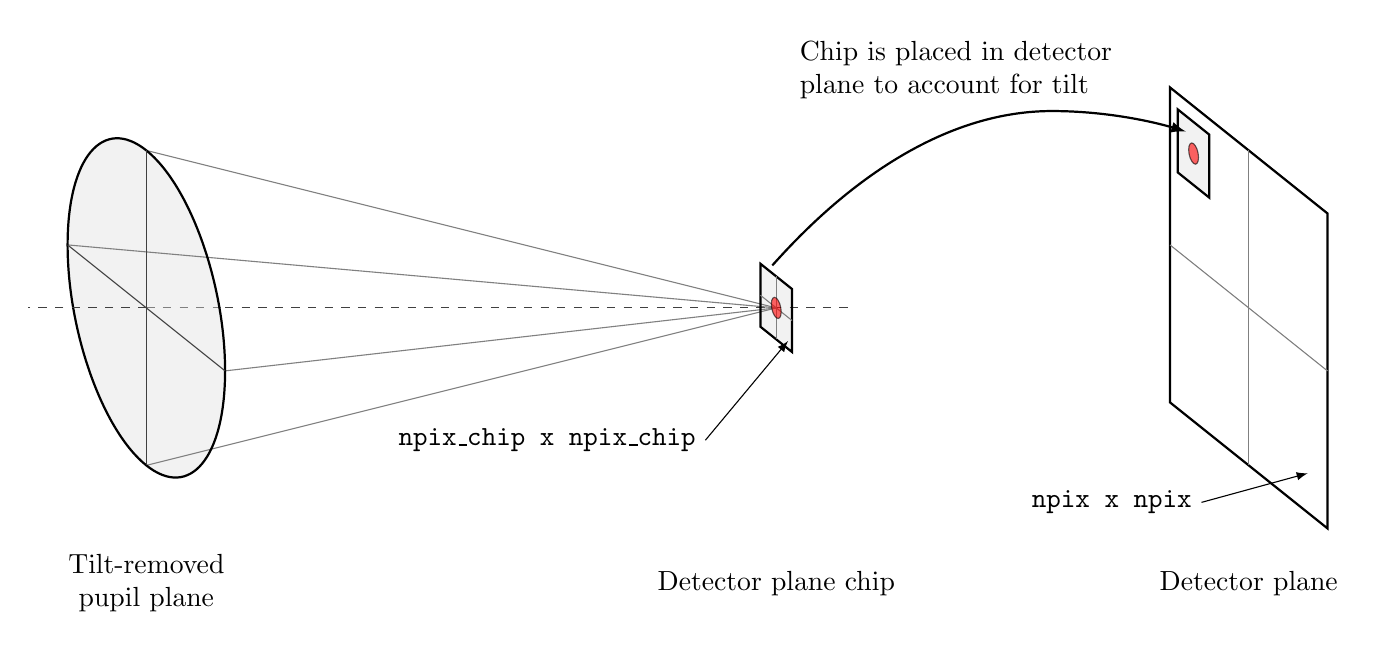
\begin{tikzpicture}[z={(1cm,0cm)},x={(0.5cm,-0.4cm)}, y={(0cm,1cm)}, scale=1]

    % constants
    \def\zimg{8}
    \def\zout{14}

    % coordinate system 
    \coordinate (0) at (0,0,0);
    \coordinate (2) at (0,0,\zimg);
   
    % optical axis
    \draw[dashed, color=gray] (0) -- +(0,0,1);
    \draw[dashed, color=darkgray] (0,0,1) -- (0,0,9);
    

    % Aperture plane
    \draw[color=gray] (-2,0,0) -- (0,0,\zimg);
    \draw[color=gray] (2,0,0) -- (0,0,\zimg);
    \draw[color=gray] (0,-2,0) -- (0,0,\zimg);
    \draw[color=gray] (0,2,0) -- (0,0,\zimg);
    
    \draw[thick, fill=gray, fill opacity=0.1] (0,0) circle [radius=2];
    \draw[color=darkgray] (-2,0,0) -- (2,0,0);
    \draw[color=darkgray] (0,-2,0) -- (0,2,0);
    
    \draw[dashed, color=darkgray] (0) -- +(0,0,-1.5);  % left side of optical axis

    \node [align=left] at (0,-3.5,0) {\begin{tabular}{c} Tilt-removed \\ pupil plane\end{tabular}};

    % Observation plane 
    \draw [thick, fill=gray, fill opacity=0.1] (-0.4,-0.4,\zimg) -- (0.4,-0.4,\zimg) -- (0.4,0.4,\zimg) -- (-0.4,0.4,\zimg) -- cycle; 
    \draw[color=gray] (-0.4,0,\zimg) -- (0.4,0,\zimg);
    \draw[color=gray] (0,-0.4,0\zimg) -- (0,0.4,\zimg);
    
    % npix
    \draw[latex-] (0.3,-0.3,\zimg) -- (1.2,-1.2,6.5);
    \node [align=center, left] at (1.2,-1.2,6.5) {\texttt{npix\_chip x npix\_chip}};


    \node [align=center] at (0,-3.5,\zimg) {Detector plane chip};

    
    % psf location
    \draw[fill=red, opacity=0.6] (0,0,\zimg) circle [radius=0.125];
   

    % Observation plane 
    \draw [thick, fill=white, fill opacity=0.1] (-2,-2,\zout) -- (2,-2,\zout) -- (2,2,\zout) -- (-2,2,\zout) -- cycle; 
    \draw[color=gray] (-2,0,\zout) -- (2,0,\zout);
    \draw[color=gray] (0,-2,0\zout) -- (0,2,\zout);

    % npix
    \draw[latex-] (1.5,-1.5,\zout) -- (1.8,-1.75,12.5);
    \node [align=center, left] at (1.8,-1.75,12.5) {\texttt{npix x npix}};

    \node [align=center] at (0,-3.5,\zout) {Detector plane};

    \draw [thick, fill=gray, fill opacity=0.1] (-1.8,1.8,\zout) -- (-1,1.8,\zout) -- (-1,1,\zout) -- (-1.8,1,\zout) -- cycle; 
    \draw[fill=red, opacity=0.6] (-1.4,1.4,\zout) circle [radius=0.125];


    \draw [-latex, thick] (-0.1,0.5,\zimg) parabola bend (-2,1.7,12.5) (-1.6,1.6,\zout);
    \node [align=center, left] at (-1.8,2.3,13.5) {\begin{tabular}{l}Chip is placed in detector\\ plane to account for tilt\end{tabular}};


\end{tikzpicture}

\end{document}
